\chapter{Máquina de Vetores Suporte}\label{chp:LABEL_CHP_2}

%exemplo: 
%caso teste:
%classe:
%atributo

Máquina de Vetores Suporte (MVS) é uma classe de algoritmos de aprendizado de máquina que surgiu nos anos 90 \cite{cortes1995support}. Hoje em dia são usadas em diversas áreas como reconhecimento de escrita, bioinformática e mineração de dados \cite{defilippo2004maquinas}. Essencialmente é um método de aprendizado supervisionado que pode ser usado para classificação binária, onde, a partir de um conjunto de dados de treinamento, a máquina aprende a classificar um caso teste como sendo de uma de duas classes; ou multi-classe, podendo classificar entre diversas classes. Para a multi-classificação o problema é subdividido em problemas binários menores. Também é possível usar uma MVS para regressão quando se quer estimar um valor ou probabilidade em vez de uma classe. 

Abordaremos nesse trabalho a máquina classificadora binária, já que é preciso entender bem como ela funciona antes de entender os outros métodos. Seguimos o fluxo de explicação abordado no livro \cite{art:LIVRO_SVM} que expõe a teoria por trás da máquina de vetores suporte de forma bem didática.

\section{Superfícies de Decisão Lineares}
Uma forma simples de se criar um classificador é através de uma superfície de decisão linear. Dado um conjunto de dados $(\bar{x}_i,y_i)$ $i\in[1,t]$, onde $t$ é o tamanho do conjunto e $\bar{x}_i \in \mathbb{R}^n$ são os atributos de cada exemplo, tambem chamado de caso teste, e $y_i \in \{ -1,+1 \}$ que é a classe do exemplo definida como $+1$ ou $-1$, se o conjunto for linearmente separável é possível criar uma superfície de decisão linear (reta, plano ou hiperplano) que separa esse conjunto de dados.

Uma vez encontrado o plano separador, a classificação fica fácil. Como podemos ver na Figura \ref{fig:LABEL_FIG_1}, se definirmos esse plano como $\bar{d}\cdot \bar{p} = \bar{d}\cdot \bar{c}$, onde $\bar{d}$ é o vetor ortogonal ao plano, $\bar{c}$ é o vetor de deslocamento de $\bar{d}$ e $\bar{p}$ são os pontos pertencentes a reta, podemos classificar um ponto $\bar{x}$ como pertencendo a uma classe usando uma função discriminante (Equação \ref{eq:LABEL_EQ_1}) onde a classe é definida pelo sinal do resultado.

\begin{equation}
f(\bar{\alpha})=sgn((\bar{\alpha}-\bar{c})\cdot\bar{d})
    \label{eq:LABEL_EQ_1}
\end{equation}

\begin{figure}
  \centering
  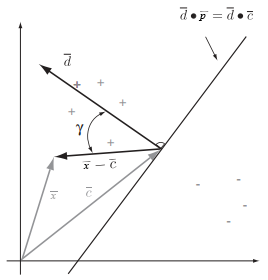
\includegraphics[width=0.4\textwidth]{imagens/svm_1.png}
  \caption{Classificação de um ponto $\bar{x}$ por uma superfície de decisão linear}
  \label{fig:LABEL_FIG_1}
\end{figure}

%silvana: definir perceptron...
%silvana: Ok!
Assumindo que nossos dados são linearmente separáveis, já sabemos qual a função discriminante, falta encontrar os parâmetros $\bar{c}$ e $\bar{d}$ que classificam corretamente esse conjunto de dados. Existem algumas formas de encontrar os parâmetros que definem essa superfície de decisão linear. Um método semelhante à máquina de vetores suporte é o perceptron \cite{art:LIVRO_SVM}. São atribuídos valores aleatórios a $\bar{c}$ e $\bar{d}$ e o perceptron classifica o conjunto de dados usando a função discriminante. A cada iteração, o perceptron corrige os valores de $\bar{c}$ e $\bar{d}$ para os dados que estiverem classificados de forma errada. Dessa forma, se o conjunto de dados for linearmente separável, o perceptron convergirá para a superfície de decisão linear.

Essa superfície separa perfeitamente os exemplos usados no treinamento, mas pode ter muitos erros para classificar outros dados. Isso ocorre porque o perceptron não tem nenhum critério para saber se a superfície é boa ou ruim. Usando a Figura \ref{fig:LABEL_FIG_2} como exemplo, suponhamos que os pontos +* e -* não estavam no conjunto de treinamento e o perceptron chegou na linha pontilhada como superfície de separação. A linha solida seria mais adequada, já que divide o espaço de forma mais justa reduzindo a chance de ter um ponto classificado errado.

\begin{figure}
  \centering
  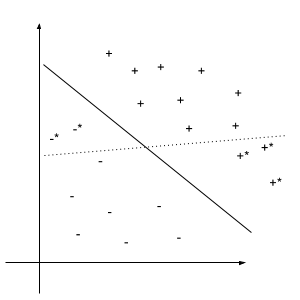
\includegraphics[width=0.4\textwidth]{imagens/svm_2.png}
  \caption{A linha sólida representa a melhor separação e a linha pontilhada representa uma separação com maior chance de erro}
  \label{fig:LABEL_FIG_2}
\end{figure}

Para encontrar essa superfície, precisamos definir hiperplanos suporte e vetores suporte. Hiperplanos suporte são as superfícies que tangenciam os dados de cada classe que queremos separar. Esses hiperplanos devem ser paralelos e a nossa superfície de decisão ótima deve se encontrar no meio desses dois hiperplanos. Vetores suporte são pontos que pertencem a esses hiperplanos de suporte.
Podemos ver na Figura \ref{fig:LABEL_FIG_3} que a superfície de decisão ótima será encontrada quando a margem entre nossos hiperplanos de suporte for máxima.

\section{Classificadores de Margem Máxima}
Classificadores de margem máxima têm como objetivo encontrar a superfície central entre duas classes de um conjunto de dados (a linha solida, na Figura \ref{fig:LABEL_FIG_2}) para minimizar a chance de erro na classificação.

\begin{figure}
  \centering
  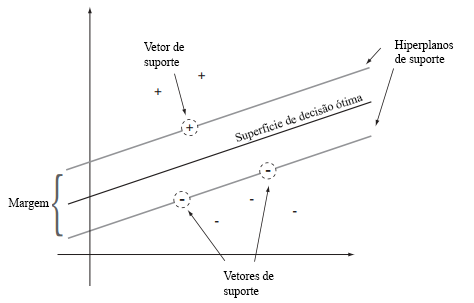
\includegraphics[width=0.7\textwidth]{imagens/svm_3.png}
  \caption{Superfície de decisão ótima e seus vetores e hiperplanos de suporte\cite{art:LIVRO_SVM}}
  \label{fig:LABEL_FIG_3}
\end{figure}

Como estamos procurando a margem máxima dado um conjunto de margens possíveis, faz sentido abordar o problema como um problema de otimização.

Formalmente, problemas de otimização são definidos como: $\underset{\bar{x}}{\min}\phi(\bar{x})$, dado que $h_i(\bar{x})\ge c_i$ $\forall \bar{x} \in \mathbb{R}^n$. Onde $\phi: \mathbb{R}^n\rightarrow \mathbb{R}$ é a função objetivo que se quer minimizar, $h_i:\mathbb{R}^n\rightarrow\mathbb{R}$ é o conjunto de funções que limitam os valores de $\phi(\bar{x})$, e $c_i$ são restrições do valor de $\bar{x}$.

Podemos então traduzir o problema de separar o conjunto de dados em um problema de otimização onde o objetivo é maximizar a distância entre os hiperplanos de suporte. Os hiperplanos suporte são hiperplanos paralelos que tangenciam os conjuntos de exemplos de cada classe e vetores suporte são pontos pertencentes a essas superfícies. Assim, o que nós queremos é a função da superfície de decisão ótima $\bar{w}^*\cdot\bar{x}=b^*$ onde a projeção entre os vetores suporte $m^*=|\bar{x}_p - \bar{x}_q|cos\gamma$, o tamanho da distancia entre os vetores multiplicado pelo coseno do ângulo entre eles, é máxima, como podemos ver na Figura \ref{fig:LABEL_FIG_4}. 

\begin{figure}
  \centering
  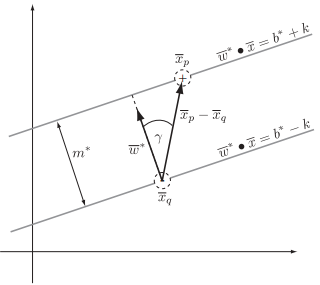
\includegraphics[width=0.6\textwidth]{imagens/svm_4.png}
  \caption{Calculando a margem $m^*$ entre os planos de suporte\cite{art:LIVRO_SVM}}
  \label{fig:LABEL_FIG_4}
\end{figure}

Para prosseguir com nossos cálculos, vamos precisar rescrever a margem ótima $m^*$ como $\frac{2k}{|\bar{w}^*|}$ (Equação \ref{eq:mEstrela}).

\begin{equation} \label{eq:mEstrela}
\begin{split}
m^* &= |\bar{x}_p-\bar{x}_q|cos\gamma\\
    &= \frac{\bar{w}^*\cdot(\bar{x}_p-\bar{x}_q)}{|\bar{w}^*|}\\
    &= \frac{\bar{w}^*\cdot\bar{x}_p-\bar{w}^*\cdot\bar{x}_q}{|\bar{w}^*|}\\
    &= \frac{(b^*+k)-(b^*-k)}{|\bar{w}^*|}\\
    &= \frac{2k}{|\bar{w}^*|}
\end{split}
\end{equation}

Queremos o vetor $\bar{w}$ que nos dê $m^*$ máximo mas para facilitar nossos cálculos mais à frente vamos reescrever nossa função objetivo como:

\begin{equation}\label{eq:funcaoObjetivo}
\begin{split}
m^*=\frac{2k}{|\bar{w}^*|} &= \max \frac{2k}{|\bar{w}|} \\
    &= \min \frac{|\bar{w}|}{2k} \\
    &= \min \frac{|\bar{w}|^2}{2k}  \\
    &= \min \frac{1}{2k} \bar{w}\cdot\bar{w}  \\
    &= \min \frac{1}{2} \bar{w}\cdot\bar{w}
\end{split}
\end{equation}

Na Função \ref{eq:funcaoObjetivo} o primeiro passo se justifica pois a maximização de uma função é igual a minimização da função inversa. O segundo passo se justifica pois o tamanho do vetor $|\bar{w}|$ é sempre positivo e a transformação de $|\bar{w}|$ para $|\bar{w}|^2$ é monotônica, então o valor de $\bar{w}$ que minimiza $|\bar{w}|$ é o mesmo que minimiza $|\bar{w}|^2$. O último passo é justificado pois a otimização não varia com a multiplicação de uma constante, assim podemos definir $k=1$ e remove-lo da equação.

Nossas restrições $h_i$ podem ser escritas como:
%Felipe: essa notação ta certa o tal que? precisa de uma chave aí?
\begin{equation}
\begin{split}
\bar{w}^*\cdot\bar{x}_i \ge b^*+k \quad \forall (\bar{x}_i,y_i)\in D \quad | \quad y_i=+1 \\
\bar{w}^*\cdot\bar{x}_i \le b^*-k \quad \forall (\bar{x}_i,y_i)\in D \quad | \quad y_i=-1 \\
\bar{w}^*\cdot\bar{x}_i \ge 1+b \quad \forall (\bar{x}_i,y_i)\in D \quad | \quad y_i=+1 \\
\bar{w}^*\cdot(-\bar{x}_i) \ge 1-b \quad \forall (\bar{x}_i,y_i)\in D \quad | \quad y_i=-1
\end{split}
\end{equation}

Essas restrições podem ser comprimidas na Equação \ref{eq:restricoesComprimidas}.

\begin{equation} \label{eq:restricoesComprimidas}
    \bar{w}^*\cdot(y_i\bar{x}_i) \ge 1+y_i b \quad \forall (\bar{x}_i,y_i)\in D
\end{equation}

Assim, um classificador por margem máxima fica definido como: dado um conjunto de dados linearmente separáveis $D=(\bar{x}_i,y_i) \subseteq \mathbb{R}^n\times\{+1,1\}$, podemos encontrar a superfície máxima de separação, $\bar{w}^*\cdot\bar{x}=b^*$, otimizando o problema $\min\phi(\bar{w},b)=\underset{\bar{w},b}{\min}\frac{1}{2}\bar{w}\cdot\bar{w}$ sujeito às restrições da Equação \ref{eq:restricoesComprimidas}.
\par

Uma máquina de vetores suporte é o problema dual do classificador de margem máxima. Podemos entender um problema dual como uma versão análoga do problema onde, ao invés de encontrar o vetor que define a superfície de separação $w$, queremos encontrar o conjunto de valores de $\bar{\alpha}$ do qual podemos inferir $w$. Para resolver esse problema dual, utilizamos a técnica dual Lagrangiana, a qual pode ser vista nos trabalhos de \cite{art:LIVRO_SVM} e \cite{art:LIVRO_KAA}.

O método de otimização Lagrangiana reescreve um problema de otimização da forma:
\begin{equation}
\underset{\bar{x}}{min}\phi(\bar{x}) \quad \text{dado que} \quad h_i(\bar{x})\ge c_i
\end{equation}
como:
\begin{equation}
\underset{\bar{\alpha}}{max} \underset{\bar{x}}{min} L(\bar{\alpha},\bar{x}) = \underset{\bar{\alpha}}{max} \underset{\bar{x}}{min}\bigg(\phi(\bar{x})-\sum_{i=1}^{l}\alpha_i g_i(\bar{x})\bigg)
    \label{eq:LABEL_EQ_7}
\end{equation}
dado que $\alpha_i\ge0$.

Para encaixarmos nosso problema no dual lagrangiano, precisamos reescrever nossas restrições como $g_i(\bar{x})=h_i(\bar{x})-c_i$. Encontrados os valores máximo de $\alpha^*$ e mínimo de $x^*$ a solução do problema dual será a mesma do problema primal, contanto que as seguintes condições se apliquem:

\begin{equation}
\begin{split}
\frac{\partial L}{\partial \bar{x}}(\bar{\alpha}^*,\bar{x})&=\bar{0}, \\
\alpha_i^*g_i(\bar{x}^*)&=\bar{0}, \\
g_i(\bar{x}^*)&\ge\bar{0} , \\
\bar{\alpha}_i^*(\bar{x}^*)&\ge\bar{0} 
\end{split}
\end{equation}

Essas condições são conhecidas como as condições de Karush-Kuhn-Tucker ou KKT, e podemos usá-las para reescrever nosso problema dependendo somente de $\bar{\alpha}$, facilitando nossa busca. Agora podemos aplicar essa técnica ao nosso problema de margem máxima, escrevendo nossa função lagrangiana como:

\begin{equation}
\begin{split}
L(\bar{\alpha},\bar{w},b) &=\phi(\bar{w},b) -  \sum_{i=1}^{l}\alpha_i g_i (\bar{w},b) \\
 &=\frac{1}{2}\bar{w}\cdot\bar{w} - \sum_{i=1}^{l}\alpha_i (y_i(\bar{w}\cdot \bar{x}_i -b)-1) \\
 &=\frac{1}{2}\bar{w}\cdot\bar{w} - \sum_{i=1}^{l}\alpha_i y_i \bar{w}\cdot \bar{x}_i + b \sum_{i=1}^{l}\alpha_i y_i + \sum_{i=1}^{l}\alpha_i\\
\end{split}
\end{equation}

Aplicando as KKTs chegamos ao nosso classificador de margem máxima dual:
\begin{equation}
    \underset{\bar{\alpha}}{max} \phi' (\bar{\alpha}) = \underset{\bar{\alpha}}{max} \Bigg( \sum_{i=1}^{l}\alpha_i - \frac{1}{2}\sum_{i=1}^{l}\sum_{j=1}^{l}\alpha_i \alpha_j y_i y_j \bar{x}_i\cdot \bar{x}_j \Bigg)
    \label{eq:EQ_Treinador_1}
\end{equation}
dado que:
\begin{equation}
    \sum_{i=1}^{l}\alpha_i y_i = 0 \quad \text{e} \quad \alpha_i \ge 0 \quad \forall  i \in \{1,l\}
    \label{eq:restricoes}
\end{equation}

Uma vez encontrado nosso $\bar{\alpha}^*$ ótimo, podemos classificar um novo ponto $\bar{x}$ com a fórmula:

\begin{equation}
    f(\bar{x}) = sgn\Bigg(
        \sum_{i=1}^{l} \alpha_i^*y_i\bar{x}_i\cdot\bar{x}
        -b^*
    \Bigg)
    \label{eq:EQ_Classificador_1}
\end{equation}

\begin{equation}
    b^* = \sum_{i=1}^{l} 
    \Bigg(
        \alpha_i^*y_i\bar{x}_i\cdot\bar{x}_{sv+} -1
    \Bigg)
    \label{eq:EQ_B_1}
\end{equation}

Onde $b^*$ representa a distância do plano à origem, $\alpha_i^*=0$ implica que $\bar{x}_i$ não influencia no resultado, $\alpha_j^*> 0$ implica que $\bar{x}_j$ é um vetor de suporte e $\bar{x}_{sv+}$ é um vetor de suporte positivo qualquer.


\section{O Truque do Kernel}
Com o que foi apresentado nas seções anteriores, conseguimos uma máquina de vetores suporte linear. Porém poucos conjuntos de dados são, na prática, linearmente separáveis. Para usar nossa máquina em conjuntos de dados que não sejam linearmente separáveis precisamos projetá-los de forma que fiquem linearmente separáveis, como na Figura \ref{fig:LABEL_FIG_5}.

\begin{figure}
  \centering
  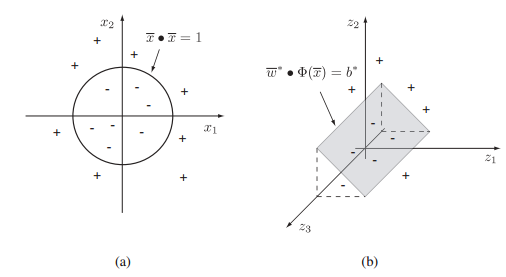
\includegraphics[width=1\textwidth]{imagens/svm_5.png}
  \caption{Em (a) não é possível separar os conjuntos de forma linear, mas transformando os dados em $\mathbb{R}^2\rightarrow \mathbb{R}^3$ em (b) conseguimos separá-los linearmente \cite{art:LIVRO_SVM}}
  \label{fig:LABEL_FIG_5}
\end{figure}

Para isso, precisamos escolher funções de projeção, $\phi:\mathbb{R}^n\rightarrow\mathbb{R}^m$, assim passamos todos nossos exemplos para um espaço de dimensão maior, na esperança que nesse espaço eles possam ser linearmente separáveis.

Podemos ver nas equações de treinamento \ref{eq:EQ_Treinador_1} e classificação \ref{eq:EQ_Classificador_1}, que sempre é avaliado o produto de dois casos teste $\bar{x}_i\cdot\bar{x}_j$, então podemos substituir $\phi(\bar{x}_i) \cdot \phi ( \bar{x}_j )$ por $k(\bar{x}_i,\bar{x}_j)$ de forma que   seja mais simples que o produto de $\phi(\bar{x})$.

Na Figura \ref{fig:LABEL_FIG_5} usamos a projeção $\phi(\bar{x})=(x_1^2,x_2^2,\sqrt{2}x_1x_2)$ e podemos simplificar seu produto (Equação \ref{eq:phiSimplificado}).

\begin{equation} \label{eq:phiSimplificado}
\begin{split}
\phi(\bar{x})\cdot \phi(\bar{y}) &= (x_1^2,x_2^2,\sqrt{2}x_1x_2) \cdot (y_1^2,y_2^2,\sqrt{2}y_1y_2) \\
&=x_1^2y_1^2+x_2^2y_2^2+2x_1x_2y_1y_2 \\
&=(x_1y_1+x_2y_2)(x_1y_1+x_2y_2) \\
&=(\bar{x}\cdot\bar{y})(\bar{x}\cdot\bar{y}) \\
&=(\bar{x}\cdot\bar{y})^2
\end{split}
\end{equation}

Chamamos essa simplificação de truque do kernel. Existe uma série de restrições que uma função tem que cumprir para ser considerada um kernel válido. Não vamos abordar aqui métodos de criação de kernels, pois é um tópico extenso, que pode ser visto em \cite{art:LIVRO_SVM}. Muitos kernels possuem uma variável livre que deve ser adaptada ao conjunto de dados estudado, podendo influenciar na sua precisão. Alguns kernels populares e suas variáveis livres podem ser vistos na Tabela \ref{tab:Kernels}.
\begin{table}
    \centering
    \caption{Kernels Populares e Suas Variáveis Livres}
    \label{tab:Kernels}
    \begin{tabular}{|c|c|c|} \hline
            Kernel & Função & Variáveis Livres \\ \hline
        Kernel Linear & $k(\bar{x},\bar{y})=\bar{x}\cdot\bar{y}$ & nenhum \\
        Kernel Homogêneo Polinomial & $k(\bar{x},\bar{y})=(\bar{x}\cdot\bar{y})^d$ & $d\ge2$ \\
        Kernel Não-Homogêneo Polinomial & $k(\bar{x},\bar{y})=(\bar{x}\cdot\bar{y}+c)^d$ & $d\ge2, c > 0$ \\
        Kernel Gaussiano & $k(\bar{x},\bar{y})=e^{-\big(\frac{|\bar{x}-\bar{y}|^2}{2\sigma^2}\big)}$ & $\sigma>0$ \\ \hline
    \end{tabular}
\end{table}

Para transformar nossa máquina de vetores suporte linear em uma máquina não linear apenas substituímos $\phi(\bar{x}_i) \cdot \phi ( \bar{x}_j )$ por $k(\bar{x}_i,\bar{x}_j)$ nas equações \ref{eq:EQ_Treinador_1}, \ref{eq:EQ_Classificador_1} e \ref{eq:EQ_B_1}.

Treinador:
\begin{equation}
    \bar{\alpha}^* = \underset{\bar{\alpha}}{argmax}{\phi}'(\bar{\alpha}) =\underset{\bar{\alpha}}{argmax} \Bigg( \sum_{i=1}^{l}\alpha_i - \frac{1}{2}\sum_{i=1}^{l}\sum_{j=1}^{l}\alpha_i \alpha_j y_i y_j k(\bar{x}_i,\bar{x}_j) \Bigg)
    \label{eq:EQ_Treinador_2}
\end{equation}

Classificador:
\begin{equation}
    f(\bar{x}) = sgn\Bigg(
        \sum_{i=1}^{l} \alpha_i^*y_i k(\bar{x}_i,\bar{x})
        -b^*
    \Bigg)
    \label{eq:EQ_Classificador_2}
\end{equation}
\begin{equation}
    b^* = \sum_{i=1}^{l}
    \Bigg(
        \alpha_i^*y_i k(\bar{x}_i,\bar{x}_{sv+})-1
    \Bigg)
    \label{eq:EQ_B_2}
\end{equation}

\section{Margem Flexível}
Conjuntos reais de dados possuem ruídos e pontos anormais que podem piorar muito a porcentagem de acertos de uma máquina de vetores suporte (Figura \ref{fig:LABEL_FIG_6}). As máquinas vistas até agora possuem margem rígida, mas também existem máquinas de vetores suporte com margem flexível que ignoram certos pontos com ruído.

Passamos a permitir que alguns pontos sejam classificados incorretamente. Definimos $\epsilon_i$ como a distância entre cada $x_i$ classificado errado e seu hiperplano de suporte, ou $0$ se o ponto estiver classificado corretamente, como pode ser visto no lado direito da Figura \ref{fig:LABEL_FIG_6}.

\begin{figure}
  \centering
  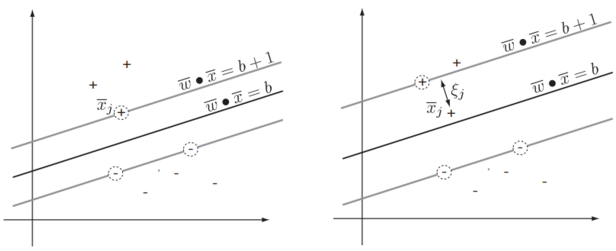
\includegraphics[width=1\textwidth]{imagens/svm_6.png}
  \caption{No exemplo da direita, ignoramos $\bar{x}_j$, que pode ser considerado ruído \cite{art:LIVRO_SVM}}
  \label{fig:LABEL_FIG_6}
\end{figure}

Para aceitar esses erros no nosso algoritmo, escolhemos uma constante $C$ que atribuímos como um peso para os erros. No problema primal, incluímos $C$ na nossa função objetivo \ref{eq:funcaoObjetivo}:

\begin{equation}
    \underset{\bar{w}, \bar{\epsilon}, b}{min}\phi(\bar{w}, \bar{\epsilon},b)
    = \underset{\bar{w}, \bar{\epsilon}, b}{min}\frac{1}{2}\bar{w}\cdot\bar{w} + C\sum_{i=1}^l \epsilon_i
    = \frac{1}{2}\bar{w}^*\cdot\bar{w}^* + C\sum_{i=1}^l \epsilon_i^*
    =m^*
\end{equation}

Queremos minimizar a função objetivo, portanto, se o peso dos erros for alto, permitimos menos erros na nossa função. No caso contrário se o peso dos erros for pequeno eles não vão influenciar tanto na função de minimização.

Concluindo,  quanto maior $C$, maior o peso dos erros e mais próximo a margem flexível fica da margem rígida. Um $C$ menor permite mais erros, fazendo com que a margem cresça e se distancie da margem rígida. No problema dual esse limite aparece como: $0\le \alpha_i \le C$

\section{Implementação}
Definimos uma máquina de vetores suporte bem robusta, capaz de classificar conjuntos de dados não lineares e suscetíveis a ruídos. A complexidade de implementação de uma MVS consiste na dificuldade de se achar os valores máximos de $\bar{\alpha}$. Existem alguns algoritmos diferentes para se chegar nesse resultado, alguns deles descritos em \cite{art:LIVRO_SVM} são apresentados a seguir.

%Felipe No livro está Gradient Ascent, não sei se essa tradução está boa
\subsection{Gradiente Ascendente}\label{sec:gradiente}
O algoritmo Gradiente Ascendente (\ref{alg:gradiente}) usa o gradiente de $\alpha$ para chegar no seu valor ótimo. O gradiente de um vetor é um vetor que aponta para a direção onde a função cresce naquele ponto. Dessa forma, podemos calcular o gradiente de $\bar{\alpha}$ em um ponto aleatório e incrementar os valores de $\bar{\alpha}$ pelo gradiente. Sabemos que chegamos no máximo local quando o gradiente for $0$, ou quando a diferença de $\bar{\alpha}$ entre as iterações é aproximadamente $0$. Nesse ponto temos o valor ótimo de $\bar{\alpha}$. Apesar de não considerarmos $b$ nessa implementação, seu valor pode ser encontrado a partir de $\bar{\alpha}$. Calculando o gradiente do nosso treinador encontrado em \ref{eq:EQ_Treinador_2} chegamos à equação \ref{eq:Gradiente}.

\begin{equation}
    \triangledown_i {\phi}'(\bar{\alpha}) = 1-y_i\sum_{j=1}^ly_j\alpha_jk(\bar{x}_j,\bar{x}_i)
    \label{eq:Gradiente}
\end{equation}

Não temos garantia de que o tamanho do gradiente não seja maior que a distância até o ponto ótimo, por isso devemos incluir uma taxa de aprendizado $\eta$ multiplicada pelo gradiente. Valores comuns de $\eta$ variam na faixa de $[0,1]$. Como o máximo da dual lagrangiana é único, podemos garantir que o algoritmo vai convergir dado um $\eta$ pequeno o suficiente.

\begin{algorithm}[h!]
\caption{Algoritmo Gradiente Ascendente}
\label{alg:gradiente}
\begin{algorithmic}[1]
\STATE $\eta>0$
\STATE $\bar{\alpha} \leftarrow \bar{0}$
\REPEAT
\STATE $\bar{\alpha_{old}} \leftarrow \bar{\alpha}$
\FOR{$i=1$ to $l$}
\STATE $\alpha_i \leftarrow a_i + \eta \triangledown_i {\phi}'(\bar{\alpha})$
\ENDFOR
\UNTIL{$\bar{\alpha}-\bar{\alpha_{old}}\approx \bar{0}$}
\RETURN $\bar{\alpha}$
\end{algorithmic}
\end{algorithm}

\subsection{Algoritmo Kernel-Adatron} \label{sec:kaa}
O problema do Gradiente Ascendente é que ele ignora as restrições de otimização \ref{eq:restricoes}, não considera o valor de $b$ e não considera uma margem flexível. O algoritmo Kernel-Adatron (\ref{alg:KAA}) resolve esses problemas. Em \cite{art:LIVRO_KAA} é explicado que a primeira restrição, $\sum_{i=1}^{l}\alpha_i y_i = 0$, só é necessária para restringir o valor de $b$ no ponto máximo. Ao fixar o valor de $b$ em zero, podemos abrir mão dessa restrição. O valor de $b$ é usado para encontrar o deslocamento da origem da nossa superfície de decisão, de forma que, fixando esse valor em zero, nos limitamos a hiperplanos que cruzem a origem no espaço de projeção. De acordo com Campbell, na prática essa generalização não prejudica os resultados quando estamos tratando de um espaço de muitas dimensões. Assim, ficamos com as restrições $\alpha_i \ge 0$ e $\alpha_i \le C$ que podem ser facilmente implementadas.

\begin{algorithm}[h!]
\caption{Algoritmo Kernel-Adatron}
\label{alg:KAA}
\begin{algorithmic}[2]
\STATE $D = \{(\bar{x_i},y_1)...(\bar{x_i},y_1)\} \subset \mathbb{R}^{n}\times \{+1,-1\}$
\STATE $\eta>0$
\STATE $C>0$
\STATE $b=0$
\STATE $\bar{\alpha} \leftarrow \bar{0}$
\REPEAT
\STATE $\bar{\alpha_{old}} \leftarrow \bar{\alpha}$
\FOR{$i=1$ to $l$}
\STATE $\alpha_i \leftarrow min\big\{C,max\big\{0,\alpha_i + \eta-\eta y_i \sum_{j=1}^l y_j \alpha_j k(\bar{x}_j,\bar{x}_i))\big\}\big\}$
\ENDFOR
\UNTIL{$\bar{\alpha}-\bar{\alpha_{old}}\approx \bar{0}$}
\RETURN $(\bar{\alpha},b)$
\end{algorithmic}
\end{algorithm}

\subsection{Quadratic Program Solver}\label{sec:quadratic}
Como a forma de se encontrar os valores de $\bar{\alpha}$ é um problema de otimização, existem métodos genéricos de otimização que ajudam nessa tarefa. Um deles é o \emph{Quadratic Program Solver} \cite{osuna1997improved}, um algoritmo que encontra os valores de um parâmetro que minimizam uma função dado um conjunto de restrições. Várias bibliotecas implementam esse algoritmo de forma que seria possível resolver a MVS sem ter que implementar o algoritmo de otimização.

\subsection{SMO: Sequential Minimal Optimization}\label{sec:smo}
Ao invés de tentar encontrar todos os valores de $\alpha$ de uma vez, o \emph{Sequential Minimal Optimization} \cite{platt1998sequential} escolhe dois pontos de treinamento, otimiza-os e vê se as restrições de KKT são válidas para o resto do conjunto de treinamento, caso contrário, escolhe outros dois pontos e continua o algoritmo. Os pontos são escolhidos de forma que um ponto respeite as restrições e o outro seja o maior violador das restrições. Dessa forma é possível provar que o algoritmo vai convergir. Isso permite uma série de otimizações mais complexas em cima das fórmulas vistas, de forma que o cálculo final fique mais eficiente.